\documentclass{report}

\usepackage[francais]{babel}
\usepackage[utf8x]{inputenc}
\usepackage[T1]{fontenc}
\usepackage[final]{pdfpages}
\usepackage{graphicx}
\usepackage{array}
\usepackage{eurosym}
\usepackage{listings}
%\usepackage{gasetex}
\title{Université de Technologie Belfort-Montbéliard\\
Projet LO41\\
Simulation de carrefours routiers intelligents}
\author{Florian Lacour\\
Michael Ayeng}

\lstdefinestyle{customc}{
  belowcaptionskip=1\baselineskip,
  xleftmargin=\parindent,
  language=C,
  showstringspaces=false,
  basicstyle=\footnotesize\ttfamily,
  keywordstyle=\bfseries\color{green!35!black},
  commentstyle=\itshape\color{purple!30!black},
  identifierstyle=\color{blue},
  stringstyle=\color{orange},
}

\lstset{escapechar=@,style=customc}

\begin{document}



\maketitle

\tableofcontents



\chapter{Introduction}
	\paragraph{}
		Dans le cadre de l'UV LO41, architectures et utilisation des systèmes d'exploitation, nous avons étés amenés à réaliser un projet reprenant différents principes vues en cours. L'objectif de celui-ci était la réalisation d'une simulation de carrefours routiers intelligents.
	\paragraph{}
		Cette simulation doit permettre la circulation de manière fluide de véhicules se déplacent de manière autonome dans un ensemble de 4 échangeurs.
	\paragraph{}
		Dans ce rapport, nous nous intéresserons dans un premier temps au cahier des charges du projet, puis aux entités mises en place afin de réaliser ce projet. Enfin, nous verrons plus en détails le fonctionnement et la communication des différentes entités constituantes de la simulation.
	
\chapter{Cahier des charges}
	\paragraph{}
	Afin de remplir les objectifs de ce projet, il nous était demandé de réaliser un programme informatique permettant la simulation d'un ensemble de 4 carrefours routiers intelligents, gérants un trafic de véhicules autonomes. Ces carrefours routiers devaient être orchestrés par un serveur-contrôleur gérant et optimisant les flux du trafic.
	\paragraph{}
	Le développement de ce programme devait être réalisé en langage C, dans un environnement Linux. La bonne gestion de la mémoire, la prise en compte des signaux et la réutilisation de principes de communications vues en cours étaient des objectifs de ce projet.
	\begin{center}
			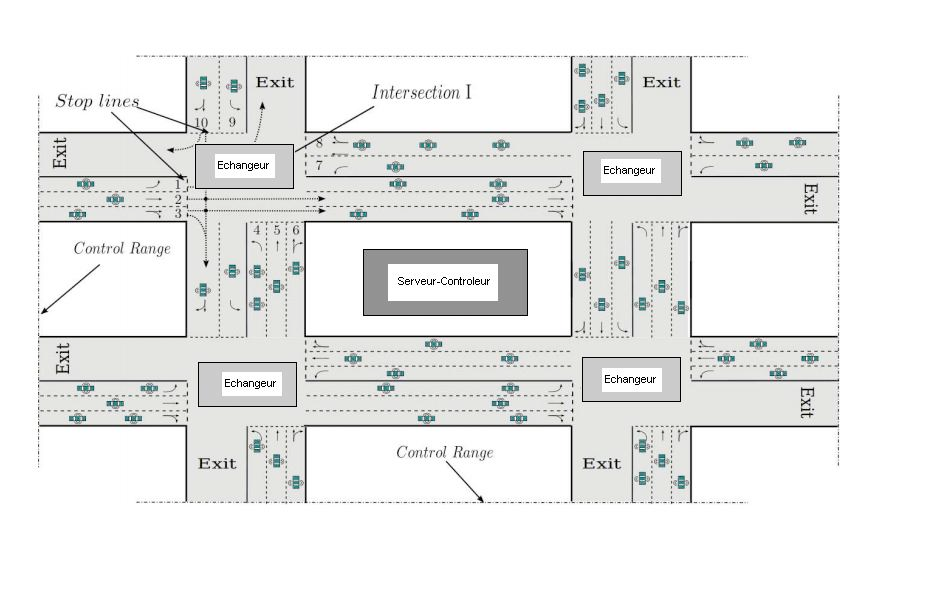
\includegraphics[scale=0.37]{simulation.png}	
			Exemple de structure routière à simuler
	\end{center}
	
	
\chapter{Présentation des entités}

	\section{Les véhicules}
	Dans cette simulation, on suppose les véhicules autonomes sont équipées d'un dispositif embarqué leurs permettant de communiquer avec l'infrastructure routière. Ces véhicules démarrent leur parcours à un échangeur et traversent la simulation jusqu'à sortir par un autre échangeur. A son arrivée aux abords d'un échangeur, le véhicule émet une requête au serveur à l'aide de son dispositif de communication, afin d'être pris en charge.
	
	\section{Les échangeurs}
	Un échangeur ne dispose pas de feux de circulation. A la place, il dispose d'une barrière virtuelle autorisant ou bloquant le parcours d'un véhicule. Ainsi, lorsqu'il en obtient l'ordre du serveur, l'échangeur va ouvrir sa barrière virtuelle et autorisé le véhicule à le traverser. L'échangeur ne peut pas autoriser plusieurs véhicules à le traverser en même temps. Lorsque le véhicule l'informe qu'il à terminer sa traversé, l'échangeur referme la barrière virtuelle.
	
	\section{Le serveur}
	Le serveur dispose d'une vue d'ensemble des échangeurs présent et dispose d'informations concernant leur état. Il connaît également la liste des véhicules qu'il doit gérer. Cette liste représente le trafic de la simulation. En permanence, le serveur est chargé d'être à l'écoute d'un véhicule souhaitant traverser un échangeur. Le serveur recherche un véhicule souhaitant traverser, en utilisant un système de priorité favorisant les véhicules dont le temps d'attente est le plus long. Lorsqu'un véhicule dont l'échangeur est disponible à été trouvé, on autorise l'échangeur à le gérer.
	
	\section{Le générateur de véhicule}
	Un générateur se charge de créer des véhicules dans la simulation. Ce générateur va paramétrer avec des valeurs aléatoires le point d'apparition et le point d'arrivée du véhicule, avec de l'ajouter à la liste de traitement du serveur.

\chapter{Fonctionnement et communication}
	
	\section{Fonctionnement}
	\paragraph{}
	La solution qui à été retenu pour la création de ce programme est l'utilisation d'un unique processus, et d'une multiplicité de threads, chacun représentant une entité de la simulation.
	
	\subsection{Le processus principal}
	
	\subsection{Le thread du serveur}
	
	\subsection{Les threads des échangeurs}
	
	\subsection{Le thread générateur de véhicule}
	
	\subsection{Les threads de véhicule}
	
	
	
	\newpage
	
	\section{Communication}
	\paragraph{}
	Le principe de sémaphore à été employé dans ce programme, afin de permettre la communication entre les différents threads. 
	\paragraph{}
	Une communication employant mutex et signaux à été mis en place pendant le développement du programme, cependant son utilisation était source de dysfonctionnement, car le nombre précis de signaux envoyés par les différentes entités était perdu.
	\paragraph{}
	L'emploi de sémaphore permet de connaître le nombre de fois qu'une notification à été envoyé, et permet ainsi aux threads d'inclure cette valeur dans leurs algorithmes de fonctionnement.
	\paragraph{}
	Tous les sémaphores sont initialisées dès le début du programme, de ce fait il est nécessaire de décider dès le début du programme d'un nombre maximum de voiture a gérer.
	
			\subsubsection{Les sémaphores des échangeurs}
			Chaque echangeur possede 2 semaphores, le premier semaphore permet de connaitre le nombre de voiture qui desire entrer dans le carrefour, le second semaphore est utiliser par la voiture pour libérer le carrefour.

			\subsubsection{Les sémaphores des véhicules}
			Les voiture posséde un semaphore afin de recevoir le signal de depart de la part de l'echangeur. 

			\subsubsection{Les sémaphores du serveur}
			\paragraph{}
			Le Serveur possede un semaphore permettant de le prevenir lorsque une voiture demande a rentrer dans l'echangeur.
		
		
	

\end{document}
